\subsection{Safety Assessment Process}
\label{subsec:process}

ARP4754A, the Guidelines for Development of Civil Aircraft and Systems~\cite{SAE:ARP4754A}, provides guidance on applying development assurance at each hierarchical level throughout the development life cycle of highly-integrated/complex aircraft systems. It has been recognized by the Federal Aviation Administration (FAA) as an acceptable method to establish the assurance process. The safety assessment process is a starting point at each hierarchical level of the development life cycle and is tightly coupled with the system development and verification processes. It is used to show compliance with certification requirements and for meeting a company's internal safety standards. 

ARP4761, the Guidelines and Methods for Conducting Safety Assessment Process on Civil Airborne Systems and Equipment~\cite{SAE:ARP4761},  identifies a systematic means to show compliance. Among the industry accepted safety assessment processes are Preliminary System Safety Assessment (PSSA) and System Safety Assessment (SSA). \janet{PSSA evaluates the system design and defines safety requirements. SSA evaluates the implemented system to show that safety requirements defined in the PSSA are in fact satisfied.} 

%PSSA performs a systematic evaluation of the system architecture and determines safety related design requirements of system components. After PSSA is completed and the components are implemented and the SSA takes place to conduct a comprehensive evaluation of the implemented system to show that safety requirements defined in the PSSA are in fact satisfied. 
	
%ARP4761, the Guidelines and Methods for Conducting Safety Assessment Process on Civil Airborne Systems and Equipment~\cite{SAE:ARP4761},  identifies a systematic means to show compliance. The guidelines presented in ARP4761 include industry accepted safety assessment processes (Functional Hazard Assessment (FHA), Preliminary System Safety Assessment (PSSA), and System Safety Assessment (SSA)), and safety analysis methods to conduct the safety assessment, 
%such as Fault Tree Analysis (FTA), Failure Modes and Effect Analysis (FMEA), and Common Cause Analysis (CCA).

%\danielle{Danielle Note: Proposal to change preceeding paragraph: The reason is because this paragraph is full of acronyms that we don't use in the paper and are not necessary to what we are describing. If someone isn't familiar with the process, these acronyms don't make sense and we don't describe them. Since our research directly applies to PSSA/SSA, these are the important things to explain. I also think a statement linking the two documents might be helpful. I previously wrote this paragraph as a replacement and I am requesting that we consider it instead of remove it.}

%To conduct the safety assessment methods described in ARP4754A, SAE Aerospace developed the ARP4761, the Guidelines and Methods for Conducting Safety Assessment Process on Civil Airborne Systems and Equipment~\cite{SAE:ARP4761}. This identifies a systematic means of showing compliance with certification standards. 

\begin{comment}
One of %these guidelines is a 
\janet{the industry accepted safety assessment processes is} 
Preliminary System Safety Assessment (PSSA). %: 
It is a systematic evaluation of the system architecture to determine safety related design requirements of system components. This assessment is conducted at multiple stages of system, component, and hardware/software design. When the PSSA is completed and the system component safety requirements are determined, the components are implemented and a System Safety Assessment (SSA) %can occur. 
\janet{can take place.}
The SSA is a comprehensive evaluation of the implemented system to show that safety requirements defined in the PSSA are in fact satisfied. 
\end{comment}

\danielle{A prerequisite of} \janet{performing the} \danielle{safety assessment is understanding how the system is intended to work, primarily focusing on the integrity of the outputs and the availability of the system.}
\janet{The safety engineers then use the acquired understanding to conduct safety analysis, construct safety analysis artifacts, and compare the results with established safety objectives and requirements.} 
%The safety engineers use this understanding to conduct the analysis and assessment process. 
\janet{Typically equipped with the domain knowledge about the system, but not detailed knowledge of how the software applications are designed, practicing safety engineers find it a time consuming and involved process to acquire the knowledge about the behavior of the software applications hosted in a system and its impact on the overall system behavior.}

%A prerequisite of performing the safety assessment of a system design is to understand how the system is intended to work, primarily focusing on the integrity of the outputs and the availability of the system. The safety engineers then use the acquired understanding to conduct safety analysis, construct safety analysis artifacts, and compare the results with established safety objectives and requirements. 

%Prior to performing the safety assessment of a system, the safety engineers are often equipped with the domain knowledge about the system, but do not necessarily have detailed knowledge of how the software applications are designed. Acquiring knowledge about the behavior of the software applications hosted in a system and its impact on the overall system behavior is typically one of the most time consuming and involved steps in the process. 

%Industry practitioners have come to realize the benefits and importance of using models to assist the safety assessment process either by augmenting the existing system design model or by building a separate safety model. A revision of the ARP4761 to include Model Based Safety Analysis (MBSA) is under way.

\janet{Industry practitioners have come to realize the benefits of using models in the safety assessment process, and a revision of the ARP4761 to include Model Based Safety Analysis (MBSA) is under way.}
% either by augmenting the existing system model or by building a separate safety model. 
Figure~\ref{fig:proposed_safety_process} presents our proposed use of a single unified model to support both system design and safety analysis. It describes both system design and safety-relevant information %. The two types of information 
\janet{that are kept distinguishable and yet are able to interact with each other.} The shared model maintains a living model that captures the current state of the system design as it moves through the development lifecycle\janet{, allowing} all participants of the ARP4754A process to be able to communicate and review the system design. Safety analysis artifacts can be generated directly from the model, %. \janet{This could} greatly improve communication and synchronization between system designer and safety engineers, \janet{and provide} %This also 
\janet{providing}
the capability to more accurately analyze complex systems.
%\danielle{, including system software applications and their impact on the overall system behavior}.

\begin{figure}[t!]
	\vspace{-0.45in}
	\centering
	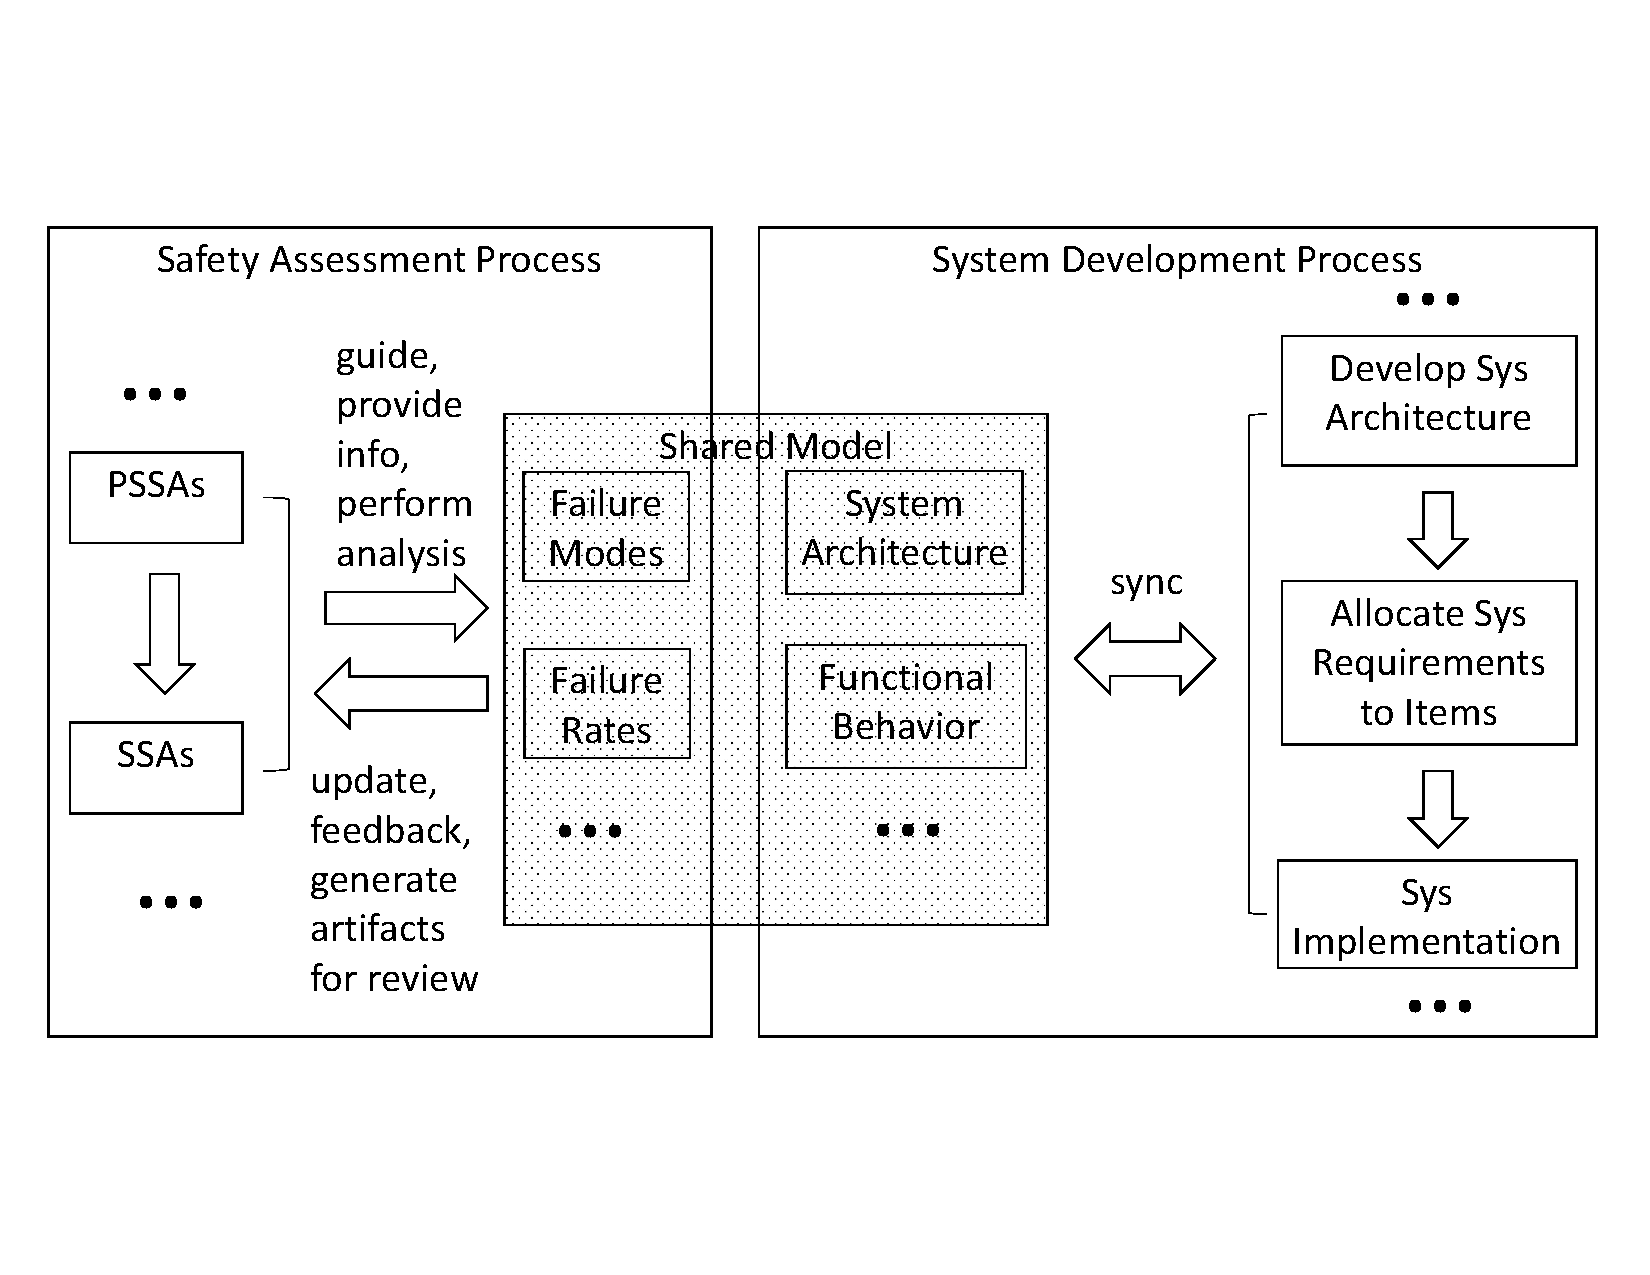
\includegraphics[trim=0 9 0 5,clip,width=0.85\textwidth]{images/safety_process.pdf}
	\vspace{-0.45in}
	\caption{Using the Shared System/Safety Model in the ARP4754A Safety Assessment Process}
	\label{fig:proposed_safety_process}
\end{figure}

\begin{comment}
 It describes both the system design information (e.g., system architecture, functional behavior) and safety-relevant information (e.g., failure modes, failure rates). The two types of information are kept distinguishable, yet are able to interact with each other. The shared model maintains a living model that captures the current state of the system design as it moves through the system development lifecycle, allowing all participants of the ARP4754A process to be able to communicate and review the system design. 

For example, the preliminary FTAs and final system FTAs (artifacts from the PSSA and SSA activities in the Safety Assessment Process) can guide and be updated from the shared model. The shared model is expected to be created and maintained in sync with the current state of the system design (including needed information from software and hardware design), and guided by the hazard and probability information from the preliminary system FTA.  The analysis results from checking the system level properties on the shared model are then used to update the preliminary system FTA. This process continues iteratively until the system safety property is satisfied with the desired fault tolerance and failure probability achieved. Consequently, the effort needed to update the final system FTA from the preliminary system FTA would be greatly reduced.


\end{comment}

\begin{comment}
When conducting the safety assessment and examining the individual subcomponents of a system, the faults and failure modes must be determined. A fault is the manifestation of an error that may lead to failure in a given component~\cite{SAE:ARP4754A}. For example, a fault in a valve may be that it is stuck closed. If this fault is active, it may cause a failure to occur. If there is no command to provide outgoing pressure, then this active fault will not cause a failure of the component to perform as intended. On the other hand, if there is such a command to provide pressure, this fault will cause failure of the valve component. The failure mode in this case is that there is a command to provide outgoing pressure, but an active fault on the valve causes it to be stuck closed. We use {\em fault} as the generic modeling keyword throughout the AADL model hierarchy and follow the definitions of these terms (error, failure, fault) throughout this description.

Many of these modes can be determined through domain knowledge and other modes are specified through the manufacturer of a given mechanical or digital component. Once the faults and failure modes are determined, the safety engineer must determine the consequence of this component failure on connected components, components that are physically located nearby, and on the system as a whole. Given that many safety critical systems are quite complex, this propagation process can be error prone and time consuming.


\janet{include a safety assessment process figure and introduce ARP4754, ARP4761 here}
\janet{describe definition for cutset here}
(The cutset is the set of primary events that must occur in order for the undesired top level event to occur)
The Primary Events are the root causes of the first level fault events.

\janet{describe what safety engineers need}

\janet{describe guidance on integration of the approach to traditional safety assessment process, e.g., system engineers model the nominal behavioral and behavioral propagations in AGREE, safety engineers add failure modes to components in safety annex, and invoke the analysis to see the effects}
\end{comment}


%\janet{J's comment: It seems to me that we could reference/mention ARP4761, FHA, PSSA etc. in a figure later in this section and briefly explain them in small-font notes that accompany the figure, but not necessary explaining them at the beginning of this section, so to avoid too much information loaded at the beginning. Therefore I commented out those descriptions for now, and revived some of our old text from the last submission.}
 %According to ARP4754, a safety critical system is a system whose safety cannot be shown solely by test, whose logic is difficult to comprehend without the aid of analytical tools, and whose failure can directly or indirectly cause significant loss of life or property~\cite{SAE:ARP4754A}. Guaranteeing safety and reliability of safety critical systems is mandatory and the process that guides it is highly standardized and controlled~\cite{RTCA:StdC,SAE:ARP4761}. ARP4761, the Guidelines and Methods for Conducting Safety Assessment Process on Civil Airborne Systems and Equipment, identifies systematic means in order to show compliance with certification standards and has been recognized by the Federal Aviation Administration (FAA) as an acceptable method to establish the assurance process.~\cite{SAE:ARP4761}. The safety assessment process is tightly coupled with the system development and verification processes and is used to show compliance with certification requirements as well as meeting a company's internal safety standards.

%ARP4754A, the Guidelines for Development of Civil Aircraft and Systems~\cite{SAE:ARP4754A}, provides guidance on applying development assurance at each hierarchical level throughout the development life cycle of highly-integrated/complex aircraft systems, and has been recognized by the Federal Aviation Administration (FAA) as an acceptable method to establish the assurance process. The safety assessment process is a starting point at each hierarchical level of the development life cycle, and is tightly coupled with the system development and verification processes. It is used to show compliance with certification requirements, and for meeting a company's internal safety standards. 

%ARP4761, the Guidelines and Methods for Conducting Safety Assessment Process on Civil Airborne Systems and Equipment~\cite{SAE:ARP4761},  identifies a systematic means to show compliance. The guidelines presented in ARP4761 include industry accepted safety assessment processes (Functional Hazard Assessment (FHA), Preliminary System Safety Assessment (PSSA), and System Safety Assessment (SSA)), and safety analysis methods to conduct the safety assessment, such as Fault Tree Analysis (FTA), Failure Modes and Effect Analysis (FMEA), and Common Cause Analysis (CCA).

%The guidelines presented in ARP4761 include the industry accepted safety assessment processes Functional Hazard Analysis (FHA), Preliminary System Safety Assessment (PSSA), and System Safety Assessment (SSA). An FHA is a comprehensive examination of aircraft functions used to identify and classify failure conditions according to severity. Early in in the development of the aircraft, the aircraft level FHA is a high level assessment of aircraft functions that establishes the safety requirements that the aircraft must meet. The system level FHA considers a failure or combination of system failures that affect an aircraft function. system level FHA is an iterative analysis and becomes more defined and fixed as the system is developed. 

%Preliminary System Safety Assessment (PSSA) is a systematic evaluation of the system architecture to determine safety related design requirements of system components. This assessment is conducted at multiple stages of system, component, and hardware/software design. As the PSSA is developed, the system level FHA is updated accordingly. When the PSSA is completed and the system component safety requirements are determined, the components are implemented and a System Safety Assessment (SSA) can occur. The SSA is a comprehensive evaluation of the implemented system to show that safety requirements defined in the PSSA are in fact satisfied. 

%A prerequisite of performing any safety assessment of a system design is to understand how the system is intended to work, primarily focusing on the relationship between component outputs and the overall behavior of the system. The safety engineers then use the acquired understanding to conduct safety analysis, construct the safety analysis artifacts, and compare the analysis results with established safety objectives and safety-related requirements. In practice, prior to performing the safety assessment of a system, the safety engineers are often equipped with the domain knowledge about the system, but do not necessarily have detailed knowledge of how the software functions are designed. Acquiring the required knowledge about the behavior and implementation of each software function in a system can be a very time consuming and involved process. For example, understanding 

%System safety analysis techniques are crucial in the development life cycle of highly integrated/complex aircraft systems and are used to show compliance with certification requirements~\cite{SAE:ARP4754A, SAE:ARP4761}. 
%A prerequisite of performing any safety assessment of a system design is to understand how the system is intended to work, primarily focusing on the relationship between component outputs and the overall behavior of the system. The safety engineers then use this information to conduct safety analysis, construct the safety analysis artifacts, and compare the analysis results with established safety objectives and safety-related requirements. 
%In practice, prior to performing the safety assessment of a system, the safety engineers are often equipped with the domain knowledge about the system, but do not necessarily have detailed knowledge of how the software applications hosted in a system are designed. Acquiring the required knowledge about the behavior and implementation of each software application in a system can be a very time consuming and involved process.
%Acquiring knowledge about the behavior of the software applications hosted in a system and its impact on the overall system behavior has shown in practice one of the most time consuming and involved step in the safety assessment process.

%For example, in a recent project it took one of our safety engineers two days to understand how the software in a Stall Warning System was intended to work. The primary task includes connecting the signal and function flows to relate the input and output signals from end-to-end and understanding the causal effect between them. This is at least as much time as was required to construct the safety analysis artifacts and perform the safety analysis itself.

%In another instance, it took a safety engineer several months to finalize the PSSA document for a Horizontal Stabilizer Control System, because of two major design revisions requiring multiple rounds of reviews with system, hardware, and software engineers to establish complete understanding of the design details.


%For example, recently a Rockwell Collins Safety Engineer performed a series of analyses on a Stall Warning System. The primary task of the safety engineer included connecting the signal and function flows to relate the input and output signals from end-to-end and understanding the causal effect between them. Once the system interactions and behavior is clear, then the safety engineer can begin to construct the safety analysis artifacts and perform the safety analysis. In cases when major design revisions occur in system development, multiple rounds of reviews with system, hardware, and software engineers must take place in order for a safety engineer to establish complete understanding of design details. These tasks are time consuming and due to the complexity of systems can also be error prone.

\begin{comment}
Industry practitioners have come to realize the benefits and importance of
using models to assist the safety assessment process (either by augmenting the existing system design model, or by building a separate safety model), and a revision of the ARP4761 to include {\em model based safety analysis} is under way.
Capturing failure modes in models and generating safety analysis artifacts directly from models could greatly improve communication and synchronization between system designer and safety engineers, and provide the ability to more accurately analyze complex systems. 

We believe that using a single unified model to conduct both system development and safety analysis can help reduce the gap in comprehending the system behavior and transferring the knowledge between the system designers and the safety analysts. It maintains a living model that captures the current state of the system design as it moves through the system development lifecycle. It also allows all participants of the ARP4754A process to be able to communicate and review the system design using a ``single source of truth.''

A model that supports both system design and safety analysis must describe both the system design information (e.g., system architecture, functional behavior) and safety-relevant information (e.g., failure modes, failure rates).  It must do this in a way that keeps the two types of information distinguishable, yet allows them to interact with each other.
\end{comment}
%\janet{J's comment: consider clarifying/replacing/complementing the following paragraph with a figure:}
%What the Safety Annex helps to provide throughout the assessment process is the ability to examine and define failure modes (the ways in which a component or system can fail) for individual system components (mechanical and digital) and then utilize behavioral propagation to determine whether these failures can cause violations of the safety requirements to occur. This can assist in understanding the system under development as well as how certain component errors contribute to both the aircraft functions and system level hazards defined in the FHA process. The nominal model and fault model are separately defined and yet interact with each  other to provide information about the system under development.

